\chapter{Lernfeld 5: Software zur Verwaltung von Daten anpassen}

\textbf{Die Schülerinnen und Schüler verfügen über die Kompetenz, Informationen mittels
    Daten abzubilden, diese Daten zu verwalten und dazu Software anzupassen.}

Die Schülerinnen und Schüler informieren sich innerhalb eines Projektes über die Abbildung
von Informationen mittels Daten. Dabei \textbf{analysieren} sie Daten hinsichtlich Herkunft, Art,
Verfügbarkeit, Datenschutz, Datensicherheit und Speicheranforderung und berücksichtigen
Datenformate und Speicherlösungen.

Sie \textbf{planen} die Anpassung einer Anwendung zur Verwaltung der Datenbestände und entwickeln Testfälle. Dabei \textbf{entscheiden} sie sich für ein Vorgehen.

Die Schülerinnen und Schüler \textbf{implementieren} die Anpassung der Anwendung, auch im
Team und erstellen eine Softwaredokumentation.

Sie testen die Funktion der Anwendung und \textbf{beurteilen} deren Eignung zur Bewältigung der
gestellten Anforderungen.

Sie \textbf{evaluieren} den Prozess der Softwareentwicklung.

% Schreibtischtest

\section{UML (Unified Modeling Language)}

\begin{figure}[H]
    \centering
    \includesvg[width=\textwidth,inkscapelatex=false]{figures/UML.drawio.svg}
    \caption{Hierarchie UML Diagramme}
\end{figure}
\FloatBarrier

\subsection{Use-Case-Diagramm}

\begin{figure}[H]
    \centering
    \includesvg[width=\textwidth,inkscapelatex=false]{figures/usecase_elemts.drawio.svg}
    \caption{Elemente im Use-Case-Diagramm}
\end{figure}
\FloatBarrier

\begin{figure}[H]
    \centering
    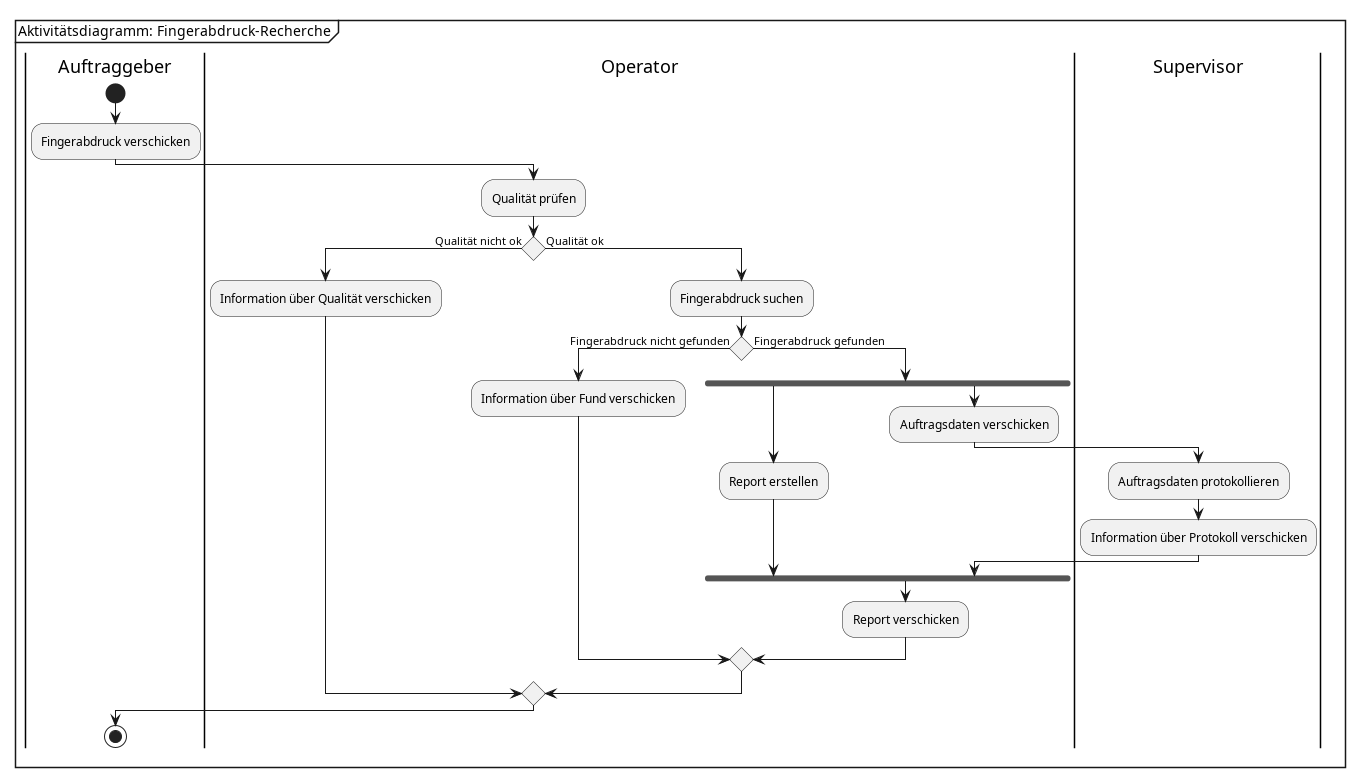
\includegraphics[width=\textwidth]{figures/activity.png}
    \caption{Beispiel Aktivitätsdiagramm}
\end{figure}